%
% File acl2018.tex
%
%% Based on the style files for ACL-2017, with some changes, which were, in turn,
%% Based on the style files for ACL-2015, with some improvements
%%  taken from the NAACL-2016 style
%% Based on the style files for ACL-2014, which were, in turn,
%% based on ACL-2013, ACL-2012, ACL-2011, ACL-2010, ACL-IJCNLP-2009,
%% EACL-2009, IJCNLP-2008...
%% Based on the style files for EACL 2006 by
%%e.agirre@ehu.es or Sergi.Balari@uab.es
%% and that of ACL 08 by Joakim Nivre and Noah Smith

\documentclass[11pt,a4paper]{article}
\usepackage[hyperref]{acl2018}
\usepackage{times}
\usepackage{latexsym}
\usepackage{mathtools}
\usepackage{amssymb}
\usepackage{url}
\usepackage{graphicx}
\graphicspath{ {images/} }

\aclfinalcopy % Uncomment this line for the final submission
%\def\aclpaperid{***} %  Enter the acl Paper ID here

%\setlength\titlebox{5cm}
% You can expand the titlebox if you need extra space
% to show all the authors. Please do not make the titlebox
% smaller than 5cm (the original size); we will check this
% in the camera-ready version and ask you to change it back.

\title{Project of the Natural Language Processing Course}

\author{Luca Di Liello \\
	University of Trento\\
	{\tt luca.diliello@studenti.unitn.it }
}


\begin{document}
\maketitle

\begin{abstract}

This document contains the instructions to prepare, implement and test a simple natural language understanding system, which will classify each word of a sentence to the corresponding IOB notation. The program has been developed using the open-source libraries OpenFST and OpenGRM, which allows the creation and the manipulation of FSA (finite state acceptors) and FST (finite state transducers) directly from the command line \cite{openfst} \cite{opengrm}. The languages used in our implementation and test phases were Bash and Python, but it's possible to use C++ instead, with similar (or probably better) results.

\end{abstract}

\section{Credits}

The software and the tecniques showed in this document were learned during the LUS course by professor Giuseppe Riccardi and professor Evgeny Stephanov. The core of the software is powered by the open-source libraries OpenFST and OpenGRM which permitted a much faster development of the project thanks to the powerful primitives to manipulate FSTs.

\section{Introduction}

One of the most important (and difficult) task in LUS is the extraction of different concepts from a given sentence. There are different ways to express a concept, but in general the problem consists in defining a map from one or more words (tokens) of a sentence to an abstract meaning representation. Lots of different notations has been created to describe concepts, and one of the most used is called IOB.

\subsection{IOB Notation}

The IOB notation (short for Inside, Outside, Beginning) is often used to tag different tokens of a sentence with a corresponding $O$, $B$ or $I$ tag, basically creating a map from words to concepts \cite{iob_notation}. $O$ tags are used to specify words that do not belong to a specific concept (e.g. stopwords), $B$ tags are those that are assigned to words that stay at the beginning of a concept and, last but not least, $I$ tags follow $B$ tags in concepts composed by more than one word. In our case, we will use a dataset containing sentences and the corresponding IOB tags, which will refer to entities about cinema and movies. In addition, for each sentence, we will have at our disposal the equivalent POS tagging and lemma list.

\subsection{OpenGRM and n-gram probability}

A $language\ model$ is a function that assigns to every word of a sentence a probability \cite{language_model}. The trivial language model is the one that assigns a probability to each word that is simply computed as the number of times that word appears divided by the total number of words in the set of sentences. Unfortunately, this model is to simple and does not lead to satisfying algorithms. An other language model is the one that applies the $chain\ rule$ to each sentence of the given dataset. In this case, the probability of each word depends on all the previous words of the same sentence. While this model is probably better than the trivial one on short sentences, it does not work well on long phrases because of the huge number of different combination of prefixes. We do not have enough data to train such a model. A simplifying assumption, called Markov assumption, consist in considering only $n$ words before the one on which we are computing the probability. The formula describing this model is the n.1:
\begin{multline}
P \big( word_{i} | word_{i-1}, ..., word_{i-n} \big)
\end{multline}
This type of model are called $n-grams$ language models. Note that usually $n$ is a small integer between 2 and 5. Taking $n = 1$ will take us back to the trivial model while taking $n$ greater than 5 will probably lead to the problem of the $chain\ rule$. The creation of a n-gram model is not difficult thanks to the OpenGRM library. OpenGRM is studied to principally offer a simple framework to build FSTs which will encode n-grams models. There is the possibility to choose between different distributions of probability of n-grams (witten-bell, katz, ...) and there is a simple and intuitive management of unknown symbols. It can be used from the command line or in C/C++ programs.

\subsection{OpenFST and WFSTs}

A weighted finite state transducer (WFST) is a direct graph with tuples of the type $(input\_label, output\_label, cost)$ on each of its edges \cite{wfst}. There are initial states and final states. The language accepted by this machine is the set of tokens such that each one identifies a route from an initial state to a final state, and the concatenation of all the input labels on the path is equal to the token itself. A single token can have more than one route from an initial state to a final state, and each path will have different cost. The total cost of each path is the sum of all costs along that path. The concatenation of all the output labels of a path is the translation of the corresponding input token. A particular version of an FST that has the input labels equal to the output labels on each edge is called finite state acceptor (FSA).
The creation and the manipulation of FSTs is a simple task thanks to the OpenFST library. Like OpenGRM, it can be used from the command line or from a C/C++ program. The first important operation permitted by the OpenGRM library is the construction of a linear FSA for each sentence of an input file. To avoid filling the folder with lots of small files, one for each sentence, they are grouped in an FAR file (short for Fst ARchive). Other significant functions comprehend the intersection, the union, the determinisation, the minimisation and the composition of FSTs. Moreover, there are tools to find the most probable token expressed by the FST through the search of the shortest path from an initial to a final state.

\section{Datasets Overview}

The training and test dataset contains sentences in the english language and, for each word, an IOB tag is given. Moreover, the lemma and the Part-of-speech tag of each word of both the training and test sets are at our disposal. The distribution of each IOB tag is showed in the histogram of Fig. 1, considering that the data refers only to the training dataset.

\begin{figure}
  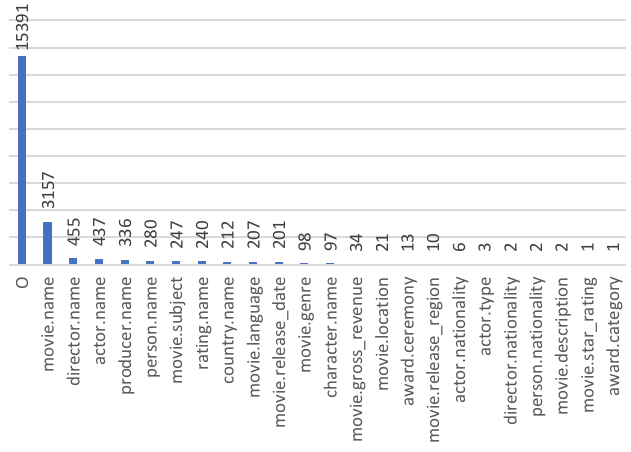
\includegraphics[scale=0.35]{concept_table.jpg}
  \caption{Concept distribution}
\end{figure}
It's interesting to see that half of the concepts appear only few times while the other half are really more frequent. In particular, the movie.name tag appears more frequently than all the others together (apart from the O tag naturally). We now take a look at the length of the sentences and the concepts in Fig. 2.
\begin{figure}
  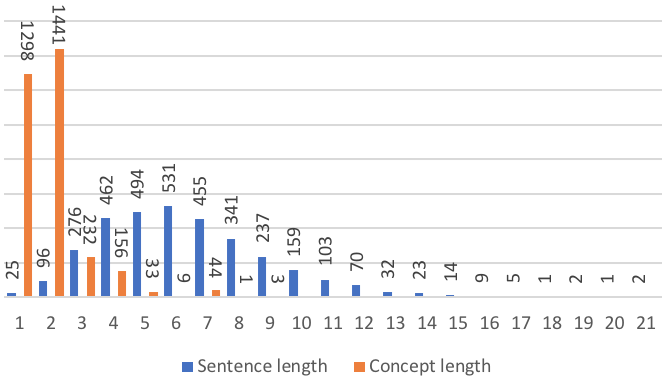
\includegraphics[scale=0.33]{length.png}
  \caption{Concept and sentence length}
\end{figure}
As you can see, the large majority of the concepts are short, composed by one or two words. There are very rare case where the length can reach 9 but the average is of 1.88 words. The length of the sentences is better distributed, with an average value of 6.42 words and some rare peaks over 15 words. Finally, some data about the size of the training and the test sets: the training set contains 3338 sentence while the test set has only 1083 sentences. This means that the ratio between training and test dimensions is about 3. The distribution of the length of sentences and concepts in the test dataset is very similar to that of the training dataset, taking in account that the total number of test sentences is reduced by 3 times.

\section{The main idea}

The core of our algorithm is based on the composition of two FSTs encoding two different probabilities.\\
The first FST will be equivalent to the formula $ P \big( token \big | concept\_tag ) $, and will be able to transduce a sequence of tokens (a sentence) in the corresponding IOB notation. This probability will be computed using the number of times a concept tag appears with a given token divided by the frequency of the single token, as showed in Formula 2. This FST will have only one state with lots of self-transitions, each of them encoding the translation of a token to a concept tag and the respective cost.
\begin{multline}
P \big( token | concept\_tag \big) = \\
C \big( token,concept\_tag \big) / C \big( concept\_tag \big)
\end{multline}
Given that an FST encodes the $cost$ of going through a specific path, the previous probability is converted in cost with the formula 3.
\begin{multline}
Cost \big( token | concept\_tag \big) = \\
- \log\big(P ( token | concept\_tag )\big)
\end{multline}

The second FST will encode the probability of a specific concept given the previous $n$ ones.
\begin{multline}
P \big( concept\_tag_n | \\
 concept\_tag_{n-1}, concept\_tag_{n-2}, ... \big)
\end{multline}
This FST, that is truly an FSA, will be created with the help of the OpenGRM library. As described in the their documentation, the available probability distributions to build the n-gram model are: witten-bell, absolute, katz, kneser-ney, presmoothed, unsmoothed. In the test section there will be results of different tests with each of this distributions. Moreover, there is the possibility to choose the deepness of the dependency of a concept tag with respect to the ones that precede. The more the number of previous concept tags on which compute the probability of the current tag, the higher the size of the equivalent FST.

The next step will consist in the composition of the previously created FSTs, being aware of the order, that is, the first left-composed to the second. As we mentioned in the introduction, the composition is a very powerful operation that should be followed by a determinisation and a minimisation to reduce the size of the result and to improve performances of next usages. What compose basically does is to merge two FSTs in such a way that if the first FST transduces token $a$ to $b$ with cost $cost_1$ and the second transduces $b$ to $c$ with cost $cost_2$, the result of the composition should transduce $a$ to $c$ with cost $ cost_1 \circledast cost_2 $.

\subsection{Improvements}

There is a simple way to improve our algorithm to perform better, that is to do some considerations on the numbers of O tags in the IOB notation of the sentences, because they are about the 75\% of the total. Given that a B tag depends on the previous O tag, if it exists, and that eventually I tags can depend on previous O tags in n-gram model with a sufficiently big $n$, one can comprehend that in this case the probabilities of B and I tags does not discriminate over the previous symbol because often it's a simple O. The idea is to substitute the O tags in the language model with the token they are representing. There is a simple way to that without applying lots of edits to the previous algorithm, that is to pre-process the input file and then to post-process the results. The preprocess will simply substitute all the O tags of the training dataset with the corresponding token. Note that the input sentences that has to be tested will not need a preprocessing phase. Finally, given the modifications we applied, the results will have B tags, I tags and tokens. The post-process will consist only in the substitution of all tokens with O tags.

\section{Test and Results}

\subsection{Base Algorithm}

\begin{figure*}
  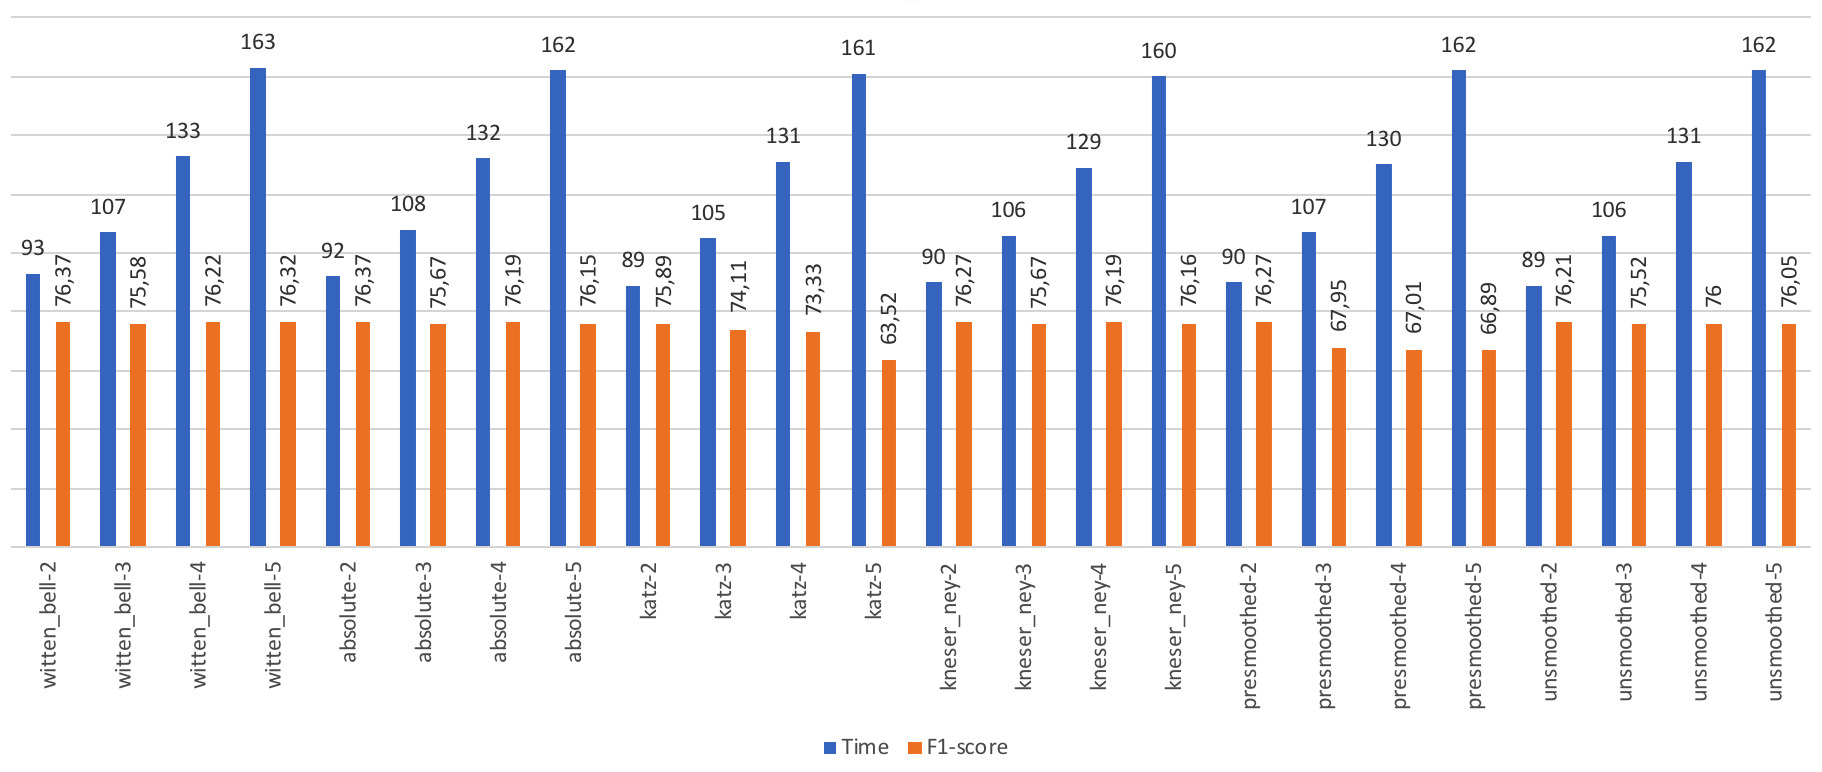
\includegraphics[width=\textwidth]{test_base.png}
  \caption{F1-score and Time of test on base case}
\end{figure*}


The graph in Fig. 3 shows the results of the base algorithm with all the different probability distributions and with and n-gram length going from 2 to 5. First some comments about the F1-score: the better tuples $(probability\ distribution, n-gram\ order)$ are the $(witten\_bell,2)$ and $(absolute,2)$. They reached an maximum F1-score of 76.37 in our test. Notice that all different combinations, apart from some particular cases, performs very similar and the variance of the results is very low. The average F1-score is of 74.25 points. In this tests, the best algorithms are those with a small n-gram order and that requires less time to execute. This is probably due to the fact that most of the concepts have a length that is less or equal than 2 tokens and that applying an n-gram model with a high order on a dataset with a strong dominant tag as O is not useful.
The time grows pretty linearly on the size of the order of the n-gram model, with all the test performed on the same machine with the same system load. The time is expressed in seconds and as you can see, our machine is able to process the test dataset in few minutes in all cases (the test dataset contains about a thousand sentences). The conclusions about this first test are that it's completely useless to use n-gram orders greater than 2 without applying the improvements we wrote about.

\subsection{Improved Algorithm}

\begin{figure*}
  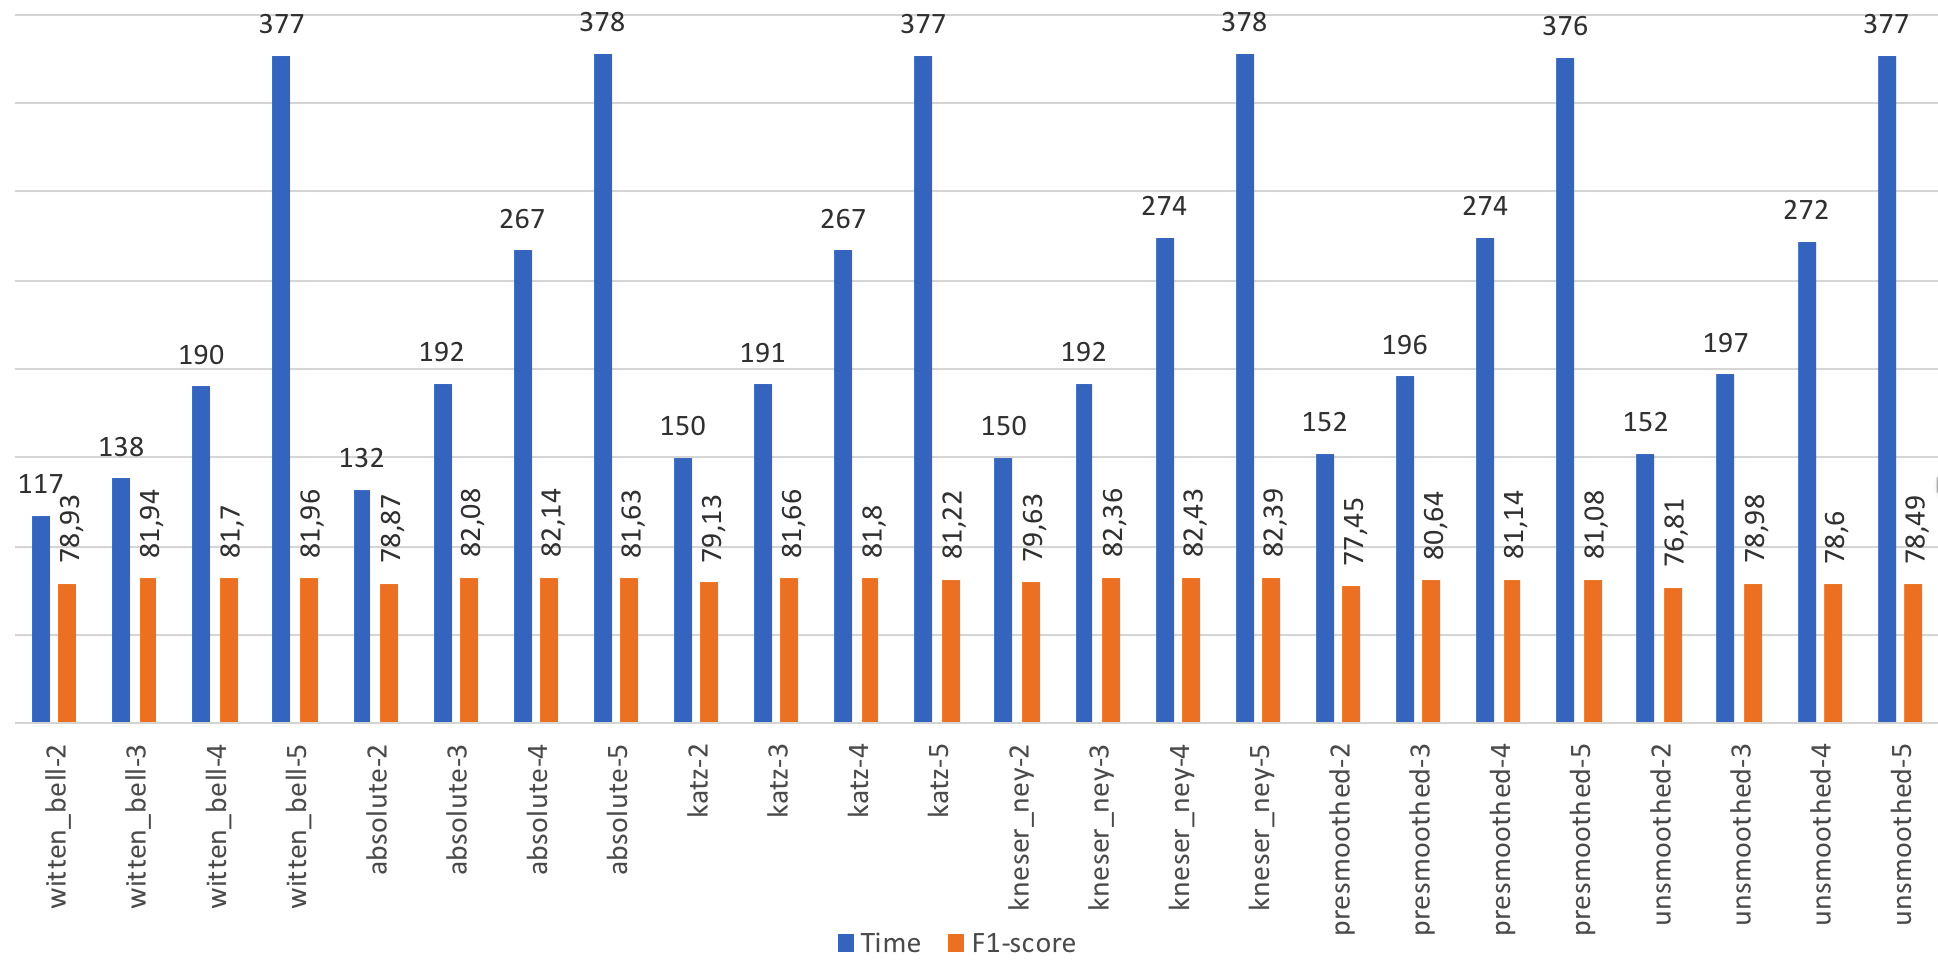
\includegraphics[width=\textwidth]{test_impr.png}
  \caption{F1-score and Time of test on improved case}
\end{figure*}

The results of the improved model, reported in Figure 4, shows an average increase of the F1-score by 6.29 points, but there are combinations, like the $(unsmoothed,2)$, that do not really perform better, with a difference in the F1-score of only 0.6. On the other side, the presmoothed distribution with a n-gram order of 5, earn more than 14 points w.r.t. the base case. In this test, the standard deviation of the F1-score results w.r.t. the base case is even lower, having all scores between 76.81 and 82.43. We will now analyse some interesting cases. First of all take a look at the time: the $witten\_bell$ distribution with an n-gram order between 2 and 3 is about the 30\% faster than all the other probability distributions. This should be taken into account in eventual large scale application, where the efficiency is a focal point. If you are more interested in maximising only the F1-score performances, probably you will note that the kneser\_ney distribution with an n-gram order of 4 has the higher F1-score of 82.43. Is it worth to use the kneser\_ney distribution only for this very small improvement of the performances with respect to the others? This should be decided by the reader.
Finally, some considerations about the time needed after having applied the improvement to the basic case. The language model built on a dataset with all the 'O's replaced by tokens is really bigger than the previous, and our tests confirmed the assumptions showing an increment of the number of edges of 17 times. This leads to test timings that are more than 2 times longer w.r.t. the basic case, especially with n-gram orders greater than 3.

\section{Error Analysis}

There are few different type of errors, each of them more or less frequent as the others:
\begin{itemize}
\item The concept is completely missed by our algorithm.
\item A concept is found but it do not really exists.
\item A concept is matched partially or it's longer than the original.
\item The type of the concept is wrong, but B and I tags were right.
\end{itemize}

Each of this error appears many times, they are not rare cases. One of the most interesting type of error is the one that starts with an I tag even if, by definition, concept must start with a B tag. With respect to the other errors, this can be easily avoided by adding some constraints on the solutions proposed by the algorithm. Given the shortest path found, check if the solution contains concepts that starts with an I tag and, if present, remove that path by applying the difference between the FST and a new linear FST containing only the solution that has to be avoided.
The other errors are more difficult to be corrected because they are the consequences of the design of our algorithm and of the small size of the training set. There are words in the test sentences that were never seen during the training phase and were treated as unknown symbols.

\section{Conclusions}

The algorithm presented in this paper has some particular advantages that has to be taken into account in eventual comparison: it is easy to be implemented and based on completely open source libraries, it's fast and does not need a particular computing power. The accuracy and the F1-score are satisfying but not the state of the art. In particular, given the presence of a dominant tag, the F1-score is a better measure for the evaluation of the performances of the system, being about 82 percentage points while the accuracy is around 93\%.

An complete example of the code is available here: \url{https://github.com/Luca1995it/LUS-project}

\bigskip


\begin{thebibliography}{2}

\bibitem{openfst}
OpenFST - Open-source library for constructing, combining, optimizing, and searching weighted finite-state transducers (FSTs). \\
\url{http://www.openfst.org/twiki/bin/view/FST/WebHome}

\bibitem{opengrm}
OpenGRM - Collection of open-source libraries for constructing, combining, applying and searching formal grammars.
\url{http://www.opengrm.org/twiki/bin/view/GRM/WebHome}

\bibitem{iob_notation}
Wikipedia - Inside-outside-beginning tagging
\url{https://en.wikipedia.org/wiki/Inside?outside?beginning_(tagging)}

\bibitem{language_model}
Wikipedia - Language Model
\url{https://en.wikipedia.org/wiki/Language_model}

\bibitem{wfst}
NYU Courant - Weighted Finite-State Transducer Definitions (Chapter 2)
\url{https://cs.nyu.edu/~mohri/pub/csl01.pdf}


\end{thebibliography}

\end{document}
